\chapter{Git}
\section{What the git is}
Github is a website that can make people able to share their ideas. People can upload and download by pushing and cloning in order. When the git saves the files, git gets the checksum with sha-1 hash before it saves. Therefore, it is difficult to lose and check the files. This checksum is a 40-character string composed of hexadecimal characters and calculated based on the contents of a file or directory structure in Git.

\section{Getting a git repository}
There are two main approaches getting a git repository. The first one take an existing project or directory it into git. The second one clone an existing git repository from another server.

If you want to move an existing project in git, you need to go to the project's directory and type:
\vspace{0.1cm}

-git init 	

-git add .

-git commit -m 'comment on the file changes'

\vspace{0.1cm}
  If you want to clone a git progect, you need to do so like this:
  \vspace{0.1cm}

-git clone https://github.com/YOUR-USERNAME/YOUR-REPOSITORY

\section{Branch}
The git branch commend is a branch administration tool. This commend can show the list of all branch, create a new branch , delete a branch and rename a branch

  If you want to create a new branch, The git branch commend can make a testing branch:
  
  - git branch testing
 \begin{figure}
 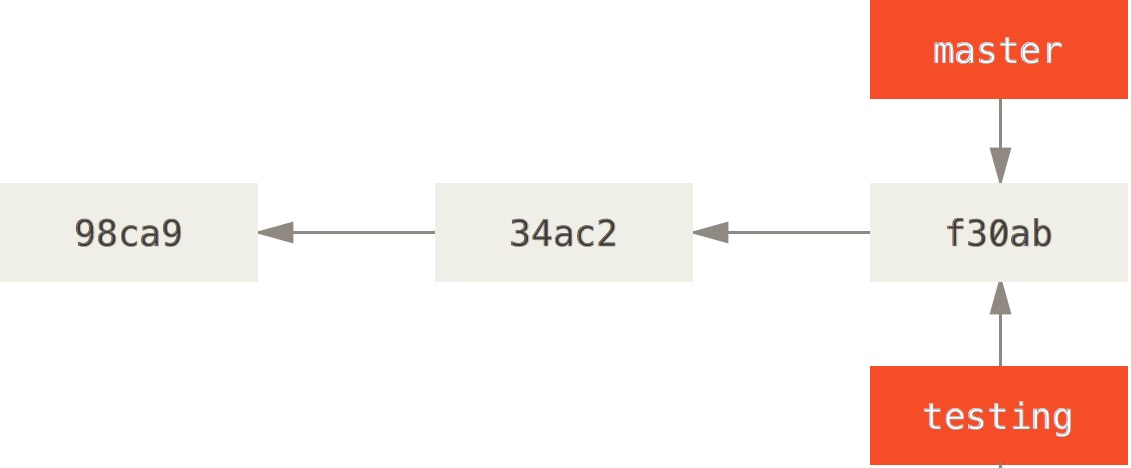
\includegraphics[width=15cm]{hit.jpg}
 \end{figure}

\vspace{2cm}

Git is differant the other virsion administration tool. Git
has a special point called HEAD. This is a pointer to local branch you'r currently on. In this case, your git is still on master branch. The git branch commend makes a new branch, dosen't move the branch. 

\section{Merge}
The git merge commend merge other branch init the branch you have checked out. If you use the "git merge <branch>" commend, the branch would merge.  